% ============================================================
%  Modeling Radioresistance and Radiotropic Fitness in Multispecies Biofilms
%  Hunter Kinder & Brett Faulkner
%  Withdrawn from the computational preprint at version 2.0; the model section of a companion experimental paper
%  This manuscript reports no live culture, recombinant/synthetic nucleic-acid
%  experiment, human or animal research, or physical irradiation experiment.
%  Preprint - not peer reviewed - August 2026
% ============================================================
\documentclass[11pt]{article}

% --- Geometry -----------------------------------------------
\usepackage[top=1in,bottom=1in,left=1.1in,right=1.1in]{geometry}

% --- Encoding & fonts ----------------------------------------
\usepackage[T1]{fontenc}
\usepackage[utf8]{inputenc}
\usepackage{lmodern}
\usepackage{microtype}

% --- Math ---------------------------------------------------
\usepackage{amsmath,amssymb,amsthm}
\usepackage{bm}

% --- Tables -------------------------------------------------
\usepackage{booktabs}
\usepackage{array}
\usepackage{tabularx}
\usepackage{longtable}
\usepackage{rotating}
\usepackage{pdflscape}

% --- Graphics & colour ----------------------------------------
\usepackage{graphicx}
\graphicspath{{figures/}}
\usepackage{xcolor}
\definecolor{linkblue}{RGB}{0,70,150}

% --- Hyperref ------------------------------------------------
\usepackage[colorlinks=true,
            linkcolor=linkblue,
            citecolor=linkblue,
            urlcolor=linkblue,
            pdftitle={Radial membrane transport under radiation-driven permeability change: a withdrawn model, kept for calibration},
            pdfauthor={Hunter Kinder, Brett Faulkner}]{hyperref}

% --- Layout ---------------------------------------------------
\usepackage{parskip}
\setlength{\parskip}{6pt}
\usepackage{setspace}
\setstretch{1.15}
\usepackage{titlesec}
\titleformat{\section}{\large\bfseries}{\thesection.}{0.5em}{}
\titleformat{\subsection}{\normalsize\bfseries}{\thesubsection}{0.5em}{}
\titlespacing{\section}{0pt}{14pt}{6pt}
\titlespacing{\subsection}{0pt}{10pt}{4pt}

% --- Floats & captions ----------------------------------------
\usepackage{caption}
\captionsetup{font=small,labelfont=bf}

% --- Line breaking --------------------------------------------
% The prose carries long \texttt{} filenames (biofilms\_potts\_jacc.jl and
% friends), which TeX will not hyphenate, so four paragraphs set overfull --
% the worst by 42pt, better than half an inch into the right margin on a
% printed page. A TeX primitive rather than a package: it lets the paragraph
% builder stretch interword space as a last resort on the lines that would
% otherwise overrun, and leaves every line that already fits untouched.
\emergencystretch=3em

% (no datetime2 in basic install)

% ============================================================
\begin{document}

\begin{center}
  {\LARGE\bfseries Radial Membrane Transport Under\\ Radiation-Driven Permeability Change}\\[10pt]
  {\large\bfseries A Model Withdrawn from the Computational Preprint,\\ Kept for the Measurements That Would Calibrate It}\\[14pt]
  {\normalsize
    \textbf{Hunter Kinder}, B.A. --- Independent Researcher, Missouri, USA\\[2pt]
    \textbf{Brett Faulkner}, B.Sc. --- Independent Researcher\\[10pt]
  }
  {\small
    \textit{Working document --- not a preprint --- September 2026}
  }
\end{center}
\vspace{4pt}
\noindent\rule{\linewidth}{0.5pt}

\section*{Status}

This text was Section~3.11, two Methods paragraphs, and one Results subsection of
\emph{Does a Dose Gradient Move Biomass Parcels?} up to version 1.2.1, and was withdrawn from
that paper at version 2.0. It is kept as the model section of a companion experimental paper.
Two things blocked it from physical interpretation in the computational paper and still do: the
coupled Julia path passes site-occupancy fractions where the rate law expects a mass
concentration, and no seconds-per-MCS mapping exists, so the dose rate it runs under is a
placeholder. The sorption term below is linear in dissolved concentration with no capacity
limit, and its rate constants have no measured values. A batch isotherm tests that assumption
directly: uptake either stays linear over the tested range or it saturates. That measurement is
the companion paper's subject, and nothing here is a result.

\section{The Model}
\subsection{Membrane Transport Under Radiation-Driven Permeability Change}
\label{sec:radiodialysis}

To model contaminant ingress through the bioreactor membrane under radiation-driven
permeability change, we introduce a minimal three-equation system coupling mobile
contaminant transport, biosorption/bioreduction, and membrane structural damage.

\emph{Radiodialysis} is a term coined for this three-equation system and is not an
established term in radiation chemistry, membrane science, or radiobiology; a targeted
search finds no scientific usage of it outside this work. The established descriptors for
the underlying phenomenon are \emph{radiolysis} (of water, into reactive oxygen species) and
the resulting \emph{lipid peroxidation}, and the literature on radiation-driven change in
membrane permeability itself uses the descriptive phrase ``radiation-induced membrane
permeability change'' (or hyperpermeability) rather than any single coined term.

\paragraph{Mobile contaminant --- cylindrical reaction-diffusion.}
The concentration $c(r,t)$ of a dissolved contaminant (e.g.\ aqueous U(VI), Cs$^+$) in the
cylindrical biofilm domain satisfies:
\begin{equation}
\frac{\partial c}{\partial t}
  = \frac{1}{r}\frac{\partial}{\partial r}\!\left(r\,D_{\mathrm{eff}}\frac{\partial c}{\partial r}\right)
  - \bigl(k_{\mathrm{ads}}X + k_{\mathrm{red}}X_{\mathrm{red}}\bigr)\,c
  + k_{\mathrm{des}}\,s
\label{eq:mobile}
\end{equation}
where $D_{\mathrm{eff}}$ is the effective diffusivity through the EPS matrix,
$k_{\mathrm{ads}}$ and $k_{\mathrm{red}}$ are the biosorption and bioreduction rate constants,
$X$ and $X_{\mathrm{red}}$ are the total and metal-reducing biomass densities, and $s(r,t)$
is the immobilised contaminant concentration (sorbed or reduced phase).
Zero-flux symmetry is imposed at $r = 0$.

\paragraph{Immobile phase --- biosorption and bioreduction.}
\begin{equation}
\frac{\partial s}{\partial t}
  = \bigl(k_{\mathrm{ads}}X + k_{\mathrm{red}}X_{\mathrm{red}}\bigr)\,c
  - \bigl(k_{\mathrm{des}} + k_{\mathrm{loss}}\bigr)\,s
\label{eq:immobile}
\end{equation}
where $k_{\mathrm{loss}}$ accounts for precipitation, co-precipitation, or export of the
immobilised fraction \cite{renslow2017}.

\paragraph{Membrane damage and radiation-driven permeability.}
Radiation progressively degrades membrane structural integrity $m(t) \in [0,1]$:
\begin{equation}
\frac{dm}{dt} = -k_{\mathrm{dam}}\,\dot{D}(R)\,m, \qquad m(0)=1
\label{eq:membrane_damage}
\end{equation}
where $\dot{D}(R)$ is the absorbed dose rate at the membrane wall ($r=R$).
The effective permeability $P_{\mathrm{eff}}$ evolves with cumulative dose
$D_{\mathrm{cum}}(t) = \dot{D}(R)\cdot t$:
\begin{equation}
P_{\mathrm{eff}}(t) = P_0\,\exp\!\bigl(\alpha_P\,D_{\mathrm{cum}}(t)\bigr)
\label{eq:peff}
\end{equation}
consistent with radiation-driven permeability enhancement observed in Nafion membranes under
ionising flux \cite{lara2023}.

\paragraph{Robin boundary condition at $r = R$.}
The membrane couples interior concentration gradient to the external reservoir $c_{\mathrm{ext}}$:
\begin{equation}
-D_{\mathrm{eff}}\left.\frac{\partial c}{\partial r}\right|_{r=R}
  = P_{\mathrm{eff}}(t)\,\bigl(c(R,t) - c_{\mathrm{ext}}\bigr)
\label{eq:robin}
\end{equation}
This is analogous to Donnan dialysis through a charged membrane \cite{aydogan2022,fox2009}.
In the present implementation, however, membrane integrity $m(t)$ and
$P_{\mathrm{eff}}(t)$ are imposed as independent functions and do not form a closed constitutive
feedback law. Equations~\ref{eq:membrane_damage}--\ref{eq:peff} should therefore be read as
candidate model components whose physical linkage remains to be selected and calibrated.


\section{The Solvers, as Executed}

\paragraph{Radiodialysis finite-volume solver (\texttt{biofilms\_radiodialysis.R}).}
Equations~\ref{eq:mobile}--\ref{eq:robin} are discretised on a one-dimensional radial grid of
$N_r=40$ points by a finite-volume method of lines and integrated with the adaptive, stiff-capable
LSODA implementation in \texttt{deSolve} \cite{soetaert2010}. The cylindrical-axis limit and the
Robin wall condition are represented explicitly in the semi-discrete operator.

\paragraph{Coupled CPM--radiodialysis diagnostic.}
The Julia file includes a forward-Euler port of the radial transport system with automatic
substepping against an explicit diffusion bound. Every ten MCS, the current implementation reduces
CPM occupancy to scalar inputs for the radial solver. Those quantities are site-occupancy fractions,
not biomass concentrations in g\,cm$^{-3}$, and the radial profile is averaged before use. The
coupled radiodialysis path is consequently retained as a numerical diagnostic and is blocked from
physical interpretation until the occupancy-to-mass mapping and membrane constitutive law are
repaired.

\section{Numerical Diagnostic, as Reported in Version 1.2.1}

\subsection{Radiodialysis Numerical Diagnostic}

The R and Julia radiodialysis implementations solve the same reaction--diffusion system with
independent time integrators. In the reported Julia run, membrane integrity decreases to
$m=0.779$ and the imposed ratio $P_{\mathrm{eff}}/P_0$ reaches $e\approx2.72$ after 100~MCS
(Figure~\ref{fig:membrane}). The latter is exact by construction from the chosen constants rather
than a fitted response. No physical MCS-to-second mapping exists, the dose-rate input is a
placeholder, and the radial coordinate is not calibrated to centimetres; these quantities are
therefore dimensionless diagnostics.

At the final snapshot, the wall concentration is approximately
$c(R,t)=0.87\,c_{\mathrm{ext}}$, while the unweighted mean over radial nodes is about
$0.024\,c_{\mathrm{ext}}$ (Figure~\ref{fig:contaminant}). The low interior value indicates limited
penetration from an initially contaminant-free interior, not depletion of a pre-existing inventory.
Because the radial biomass profile is averaged before use and site occupancy is passed where the
rate law expects mass concentration, this path remains blocked from physical interpretation.

\begin{figure}[htbp]
\centering
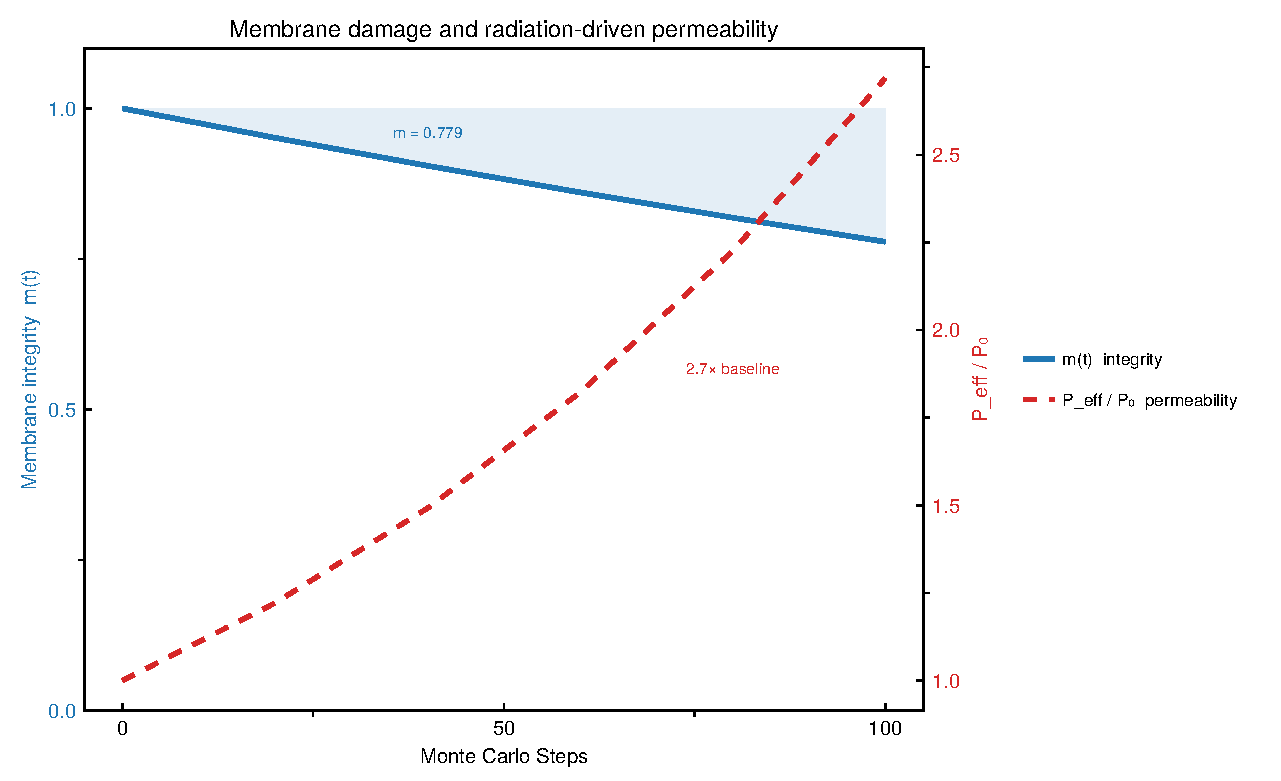
\includegraphics[width=0.88\linewidth]{fig3_membrane_transport}
\caption{Independent imposed laws for membrane integrity $m(t)$ and normalised permeability
$P_{\mathrm{eff}}(t)/P_0$ over 100~MCS. The horizontal axis is not calibrated time, and the two
curves are not a closed membrane-feedback law.}
\label{fig:membrane}
\end{figure}

\begin{figure}[htbp]
\centering
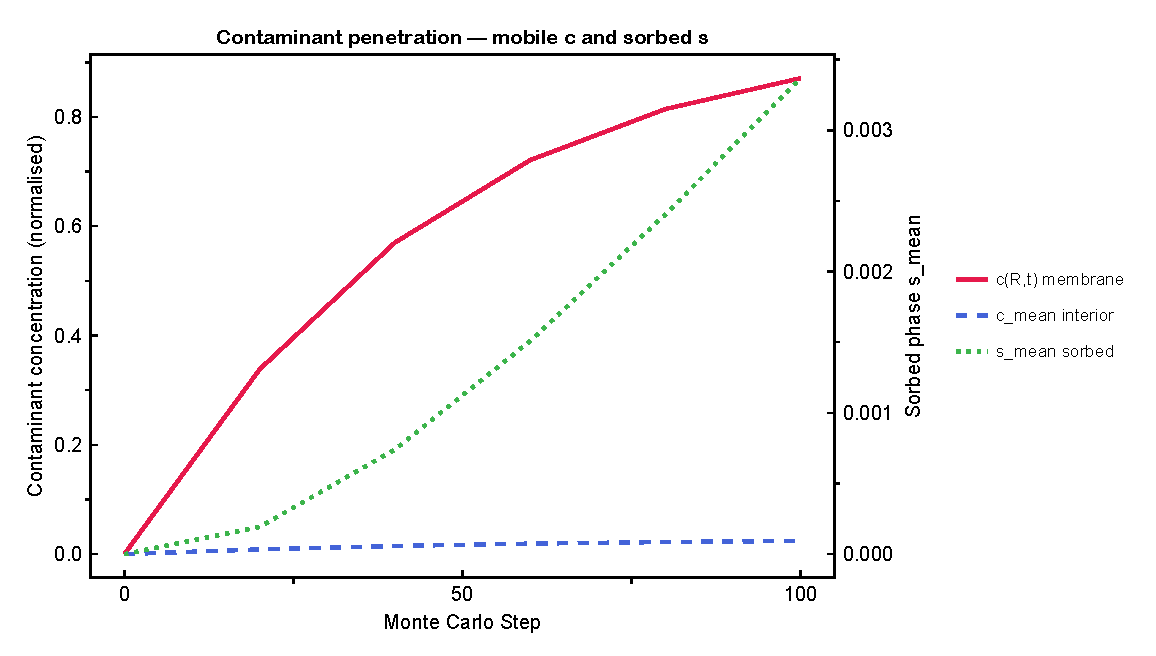
\includegraphics[width=0.88\linewidth]{fig4_contaminant_penetration}
\caption{Dimensionless mobile and sorbed contaminant diagnostics over 100~MCS. The near-zero
interior mean reflects limited penetration from the initially clean interior and must not be read as
percentage removal. The sorbed phase uses its own display scale.}
\label{fig:contaminant}
\end{figure}

\begin{thebibliography}{5}
\bibitem{soetaert2010}
Soetaert, K., Petzoldt, T., Setzer, R.W. (2010).
Solving differential equations in R: package deSolve.
\textit{Journal of Statistical Software}, 33(9), 1--25.
\url{https://doi.org/10.18637/jss.v033.i09}
\bibitem{renslow2017}
Renslow, R.S., et al. (2017).
Modeling biofilm-mediated uranium immobilization in porous media.
\textit{Water Research}, 109, 120--130.
\url{https://doi.org/10.1016/j.watres.2016.11.038}
\bibitem{lara2023}
Lara, D., et al. (2023).
Ionizing radiation effects on proton exchange membrane permeability and selectivity.
\textit{Membranes}, 13(4), 412.
\url{https://doi.org/10.3390/membranes13040412}
\bibitem{aydogan2022}
Aydogan Gokturk, P., Sujanani, R., Qian, J., Wang, L., Freyman, J.L., Bhatt, A.D.,
Freeman, B.D., Bhave, R., Boudouris, B.W., Phillip, W.A. (2022).
Donnan dialysis of monovalent ions across a cation exchange membrane.
\textit{Nature Communications}, 13, 5258.
\url{https://doi.org/10.1038/s41467-022-32930-9}
\bibitem{fox2009}
Fox, E.B., et al. (2009).
Radiation effects on Nafion$^{\circledR}$ membrane properties.
\textit{Savannah River National Laboratory Technical Report}, SRNL-STI-2009-00053.
\end{thebibliography}

\end{document}
